\PassOptionsToPackage{expansion=false}{microtype}

\documentclass{bmstu}

\usepackage{graphicx}
\graphicspath{{images/}}

\usepackage{float}

\bibliography{biblio}

\begin{document}

\makecourseworktitle
{Информатика и системы управления}
{Программное обеспечение ЭВМ и информационные технологии}
{Конструктор из геометрических примитивов}
{М.А. Семенчук/ИУ7-53Б}
{Д.А. Шибанова}
{}{}{}

\maketableofcontents

\begin{definitions}
	\definition{Рендеринг}{}
\end{definitions}
\begin{abbreviations}
	\definition{GI}{global illumination (глобальное освещение)}
	\definition{ПО}{программное обеспечение}
	\definition{ЦП (CPU)}{центральный процессор (central proccesing unit)}
	\definition{ОЗУ (RAM)}{оперативное запоминающее устройство (random access memory)}
	\definition{ГП (GPU)}{графический процессор (graphics proccesing unit)}
	\definition{}{}
\end{abbreviations}

\chapter*{ВВЕДЕНИЕ}
\addcontentsline{toc}{chapter}{ВВЕДЕНИЕ}

Компьютерная графика стала неотъемлемой частью современного мира и с каждым годом находит свое применения все в новых аспектах жизни. Она применяется в кинематографе, игровой индустрии, архитектура, медицине и других областях.

Алгоритм трассировка лучей в последние годы активно применяется в компьютерной графике. В связи с этим производители графических карт (GPU) начали добавлять в свои устройства ядра, специализирующиеся на трассировке лучей (RT-ядра). В стороне не остались разработчики графических API и библиотек, которые активно добавляют в свои продукты поддержку этой технологии. Известными примерами могут стать DirectX Ray Tracing (DXR), Vulkan RTX, CUDA/OptiX и другие. Многосторонняя поддержка этой технологии позволяет создавать все более фотореалистичные изображения с большим разрешением и лучшим качеством.

\textbf{Целью} данной работы является разработка ПО для визуализации трехмерных сцен, состояющих из геометрических примитивов, а также проведения исследования для тестирования производительности разработанного ПО.

Для достижения поставленной цели необходимо выполнить следующие \textbf{задачи}:
\begin{itemize}
    \item выбрать алгоритм генерации изображения, модель освещения и затенения;
    \item описать доступные для размещения на сцене модели и формализовать их;
    \item построить схемы алгоритмов;
    \item выбрать средства реализации (платформу, язык программирования, графическую библиотеку, GUI библиотеку);
    \item реализовать спроектированное ПО с помощью выбранных средств;
    \item провести исследование производительноси разработанного ПО.
\end{itemize}

\cite{nvidia}
\chapter{Аналитический раздел}

% \section{Методы рендеринга трехмерных сцен}
% \section{Анализ предметной области} % Камера, сцена, свет


\section{Трассировка лучей}
Трассировка лучей (от англ. Ray tracing) --- это метод рендеринга, который позволяет реалистично имитировать освещение среды за счет использования физически корректной модели поведения света. Распространяясь по сцене и взаимодействую с ее объектами, свет может отражаться, преломляться, поглощаться и рассеиваться.

\subsection{Алгоритм прямой трассировки лучей}
Главная идея, лежащая в основе алгоритма прямой трассировки лучей, заключается в том, что наблюдатель видит объекты посредством испускаемого источниками света, который многократно отражаясь, согласно законам оптики, доходит до глаз наблюдателя. Метод прямой трассировки предполагает построения траекторий лучей от всех источников освещения ко всем точкам всех объектов сцены, лучи отражаются, преломляются или проходят сквозь него и в результате достигает наблюдателя. Если объект не является отражающим или прозрачным, то траектория луча на этой точке обрывается.
\begin{figure}[H]
	\centering
	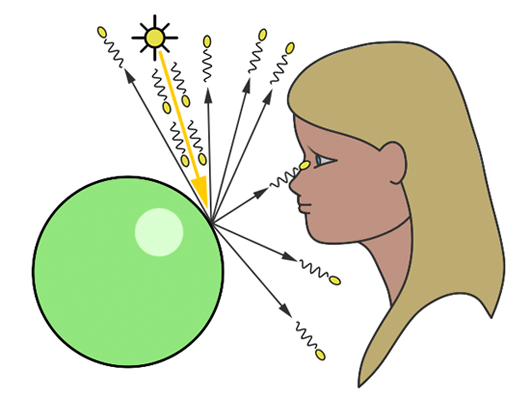
\includegraphics[width=0.8\textwidth]{forward_ray_tracing.png}
	\caption{Алгоритм прямой трассировки лучей}
\end{figure}
Основным недостатком этого алгоритма является излишне большое число рассматриваемых лучей, приводящее с существенным затратам вычислительных мощностей, так как лишь малая часть лучей достигает точки наблюдения. Однако данный алгоритм имитирует реальное поведение света и применяется в задачах, в которых точность важнее скорости (оптика и фотоника, расчет освещенности помещения и тд).

\subsection{Алгоритм обратной трассировки лучей}
На отображение сцены влияют только лучи, достигшие наблюдателя. Благодаря тому, что свет имеет особенность распространяться одинаково в обоих направлениях, можно искусственно поменять направления лучей на противоположное, и испускать лучи из точки наблюдения. Это позволяет рассматривать исключительно лучи, которые гарантированно попадут в камеру. Данный метод, основанный на испускании лучей от камеры к объектам сцены, называется обратной трассировкой лучей. Данный подход позволяет существенно сократить количество обрабатываемых лучей и обеспечить более эффективное формирование изображений при приемлемой степени физической достоверности.

\begin{figure}[H]
	\centering
	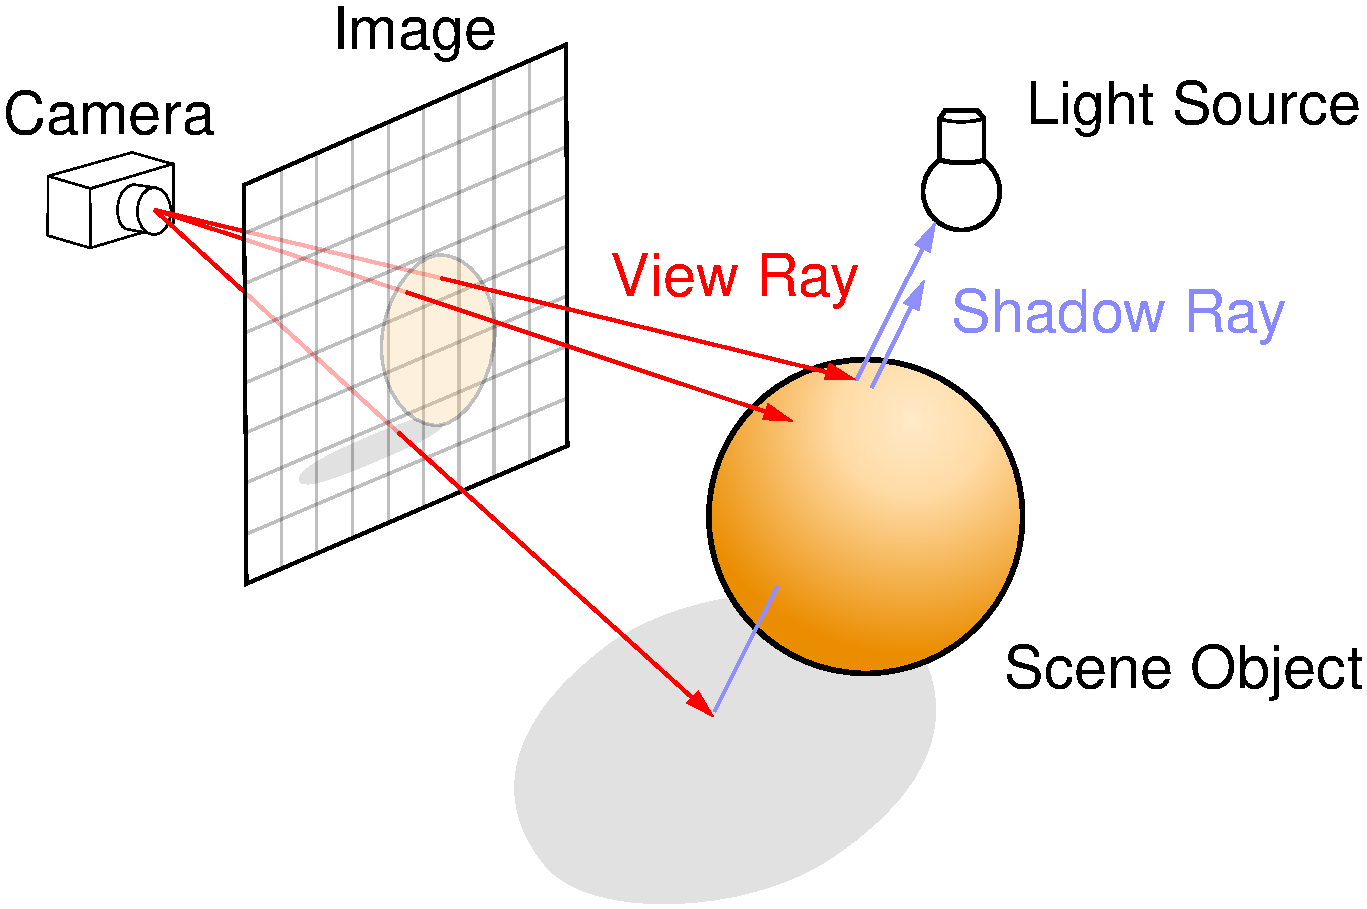
\includegraphics[width=0.8\textwidth]{backward_ray_tracing.pdf}
	\caption{Алгоритм обратной трассировки лучей}
\end{figure}

\subsection{Выбор алгоритма}

\begin{tabular}{|c|c|c|}
	\hline
	Алгоритм & Быстродействие & Реалистичность \\ 
	\hline
	Прямая трассировка лучей & Низкое & Высокая \\ 
	Обратная трассировка лучей & Среднее & Среднее \\ 
	\hline
\end{tabular}

В качестве алгоритма рендеринга был выбран метод обратной трассировки лучей, так как для поставленной задачи не требуется полная физическая корректность модели, а также важна производительность, учитывая, что программа будет выполняться на центральном, а не графическом процессоре.


\section{Анализ моделей освещения}
Свет при взаимодействии с поверхностью может быть отражен, поглощен или преломлен. Часть световой энергии поглощается поверхностью и преобразуется в тепло. Отраженный и преломленный свет делают объект видимым для наблюдателя. Если весь падающий свет будет поглощен поверхностью объекта, он будет невидимым (абсолютное черное тело).

Все модели освещения делятся на два вида: глобальные и локальные. Глобальные модели учитывают возможности отражения и преломления света от объектов, не являющихся прямыми источниками освещения, поэтому они требуют значительных вычислительных затрат. Например, прозрачные поверхности должны позволять просматривать объекты за ними, на поверхностях возможно появление таких явлений, как рефлексы. Глобальные модели освещения основываются на том, что видимость и затенения связаны между собой: яркость точки поверхности определяется распределением яркости по всем остальным поверхностям, видимым из этой точки. Так можно моделировать шероховатость и свойства отражения реальных материалов, освещение многократно отраженным светом и связанные с ним цветовые эффекты.

Существуют более простые, локальные модели освещения, которые учитывают только свет от источника. Они вычисляют интенсивность, цвет и дальнейшее распределение света на поверхности, но не учитывают перенос света между объектами. Изображение формируется в результате отражения, падающего на поверхность объектов света, интенсивность и цвет которого необходимо рассчитать. Фоновое освещение определяет цвет объекта в тени или при отсутствии явных источников освещения. Его интенсивность постоянна, а также равномерно распределена по всему пространству.
Выделяют две основные модели локального освещения: модель Ламберта и модель Фонга.

\subsection{Модель освещения Ламберта}
Модель Ламберта описывает идеальную "матовую" диффузную поверхность. Интенсивность отраженного света подчиняется закону косинусов Ламберта, согласно которому отраженное излучение одинаково во всех направлениях. При этом положение и угол обзора наблюдателя не имеют значения, т.к. диффузно отраженный свет рассеивается равномерно во всех направлениях.

\begin{figure}[H]
	\centering
	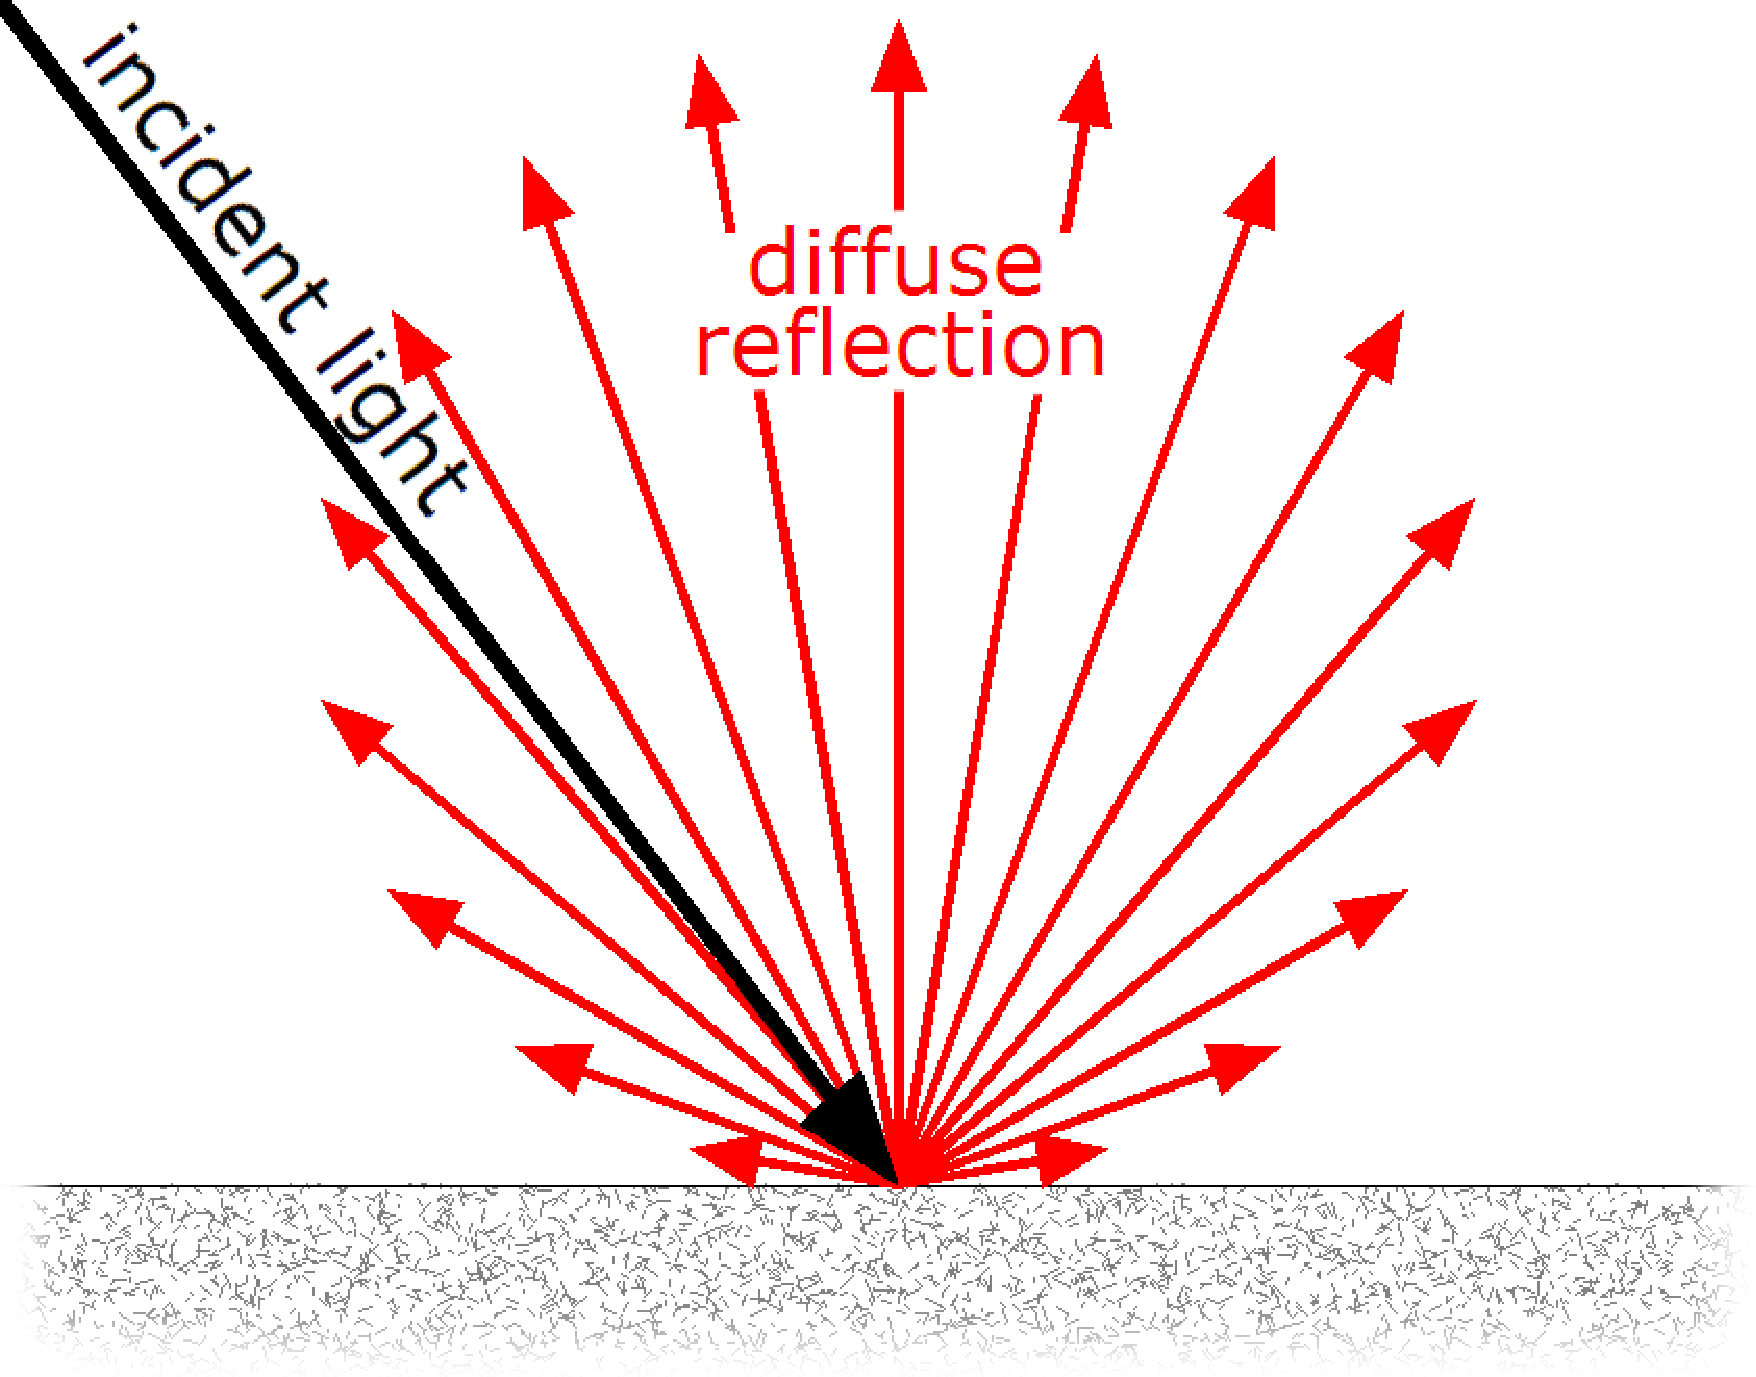
\includegraphics[width=0.8\textwidth]{lambert.pdf}
	\caption{Схема диффузного отражения Ламберта}
\end{figure}


\subsection*{Модель освещения Фонга}
\subsection*{Модель освещения Блинна-Фонга}


\subsection{Взаимодействие света с поверхностью}
\section{Обзор геометрических примитивов}


\chapter{Конструкторский раздел}

В этом разделе будут рассмотрены алгоритмы, выбранные для построения изображения, а также спроектированна диаграмма классов приложения.

\section{Алгоритм построения изображений}
В качестве средства описания алгоритма построения изображения будет использоваться диаграмма IDEF0.

Построение изображений в компьютерной графике в контексте диаграммы IDEF0 определяется следующими параметрами:

\noindent \textbf{Описание входных данных}
\begin{itemize}
    \item Объекты определяются геометрией, положением и ориентацией и свойствами материала (цвет, текстуры, нормали);
    \item Камера определяется проекцинными параметрами (перспективная, ортографическая), положением и ориентацией;
    \item Источники освещения определяются типом (направленный, точечный и др.) , положением и ориентацией (для направленных), цветом и интенсивностью.
\end{itemize}

\noindent \textbf{Описание элементов управления}
\begin{itemize}
    \item Алгоритм рендеринга: растеризация, трассировка лучей, трассировка пути, ray marching;
    \item Параметры рендеринга: разрешение получаемого изображения, максимальное число переотражений луча, количество сэмплов на пиксель;
    \item Модель освещения: локальная (Фонг, Блинн-Фонг) или глобальная (PBR\cite{pbr_book});
    \item Способ затенения: простое, по Гуро, по Фонгу.
\end{itemize}

\noindent \textbf{Описание механизмов}
\begin{itemize}
    \item Аппаратное обеспечение (CPU, RAM, GPU + VRAM);
    \item Графический API (OpenGL, Vulkan, DirectX, Metal и др.);
    \item Библиотека для окна и ввода (GLFW, SDL, SFML и др.).
    \item Язык программирования (C++, Python, C\#, Java и др.);
\end{itemize}

\noindent \textbf{Выходными данными} является сгенерированный кадр.

Общий алгоритм генерация изображений представлен на рисунке \ref{fig:IDEF0_general}.
\begin{figure}[H]
    \centering
    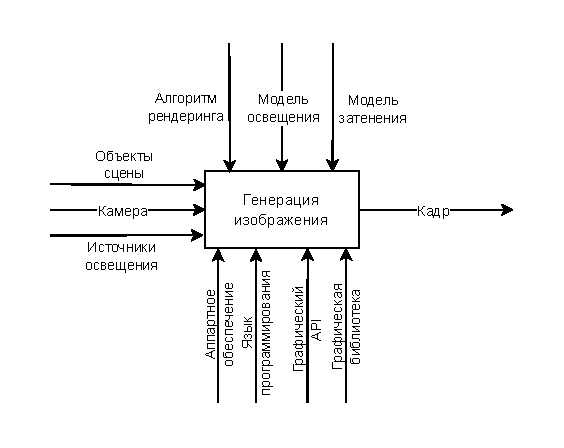
\includegraphics[width=1\textwidth]{IDEF0_general.pdf}
    \caption{IDEF0 диаграмма общего алгоритма построения изображения}
    \label{fig:IDEF0_general}
\end{figure}

Выбранный для реализации алгоритм построения изображений с конкретными методами, моделями и инструментами представлен на рисунке \ref{fig:IDEF0_specific}.
\begin{figure}[H]
    \centering
    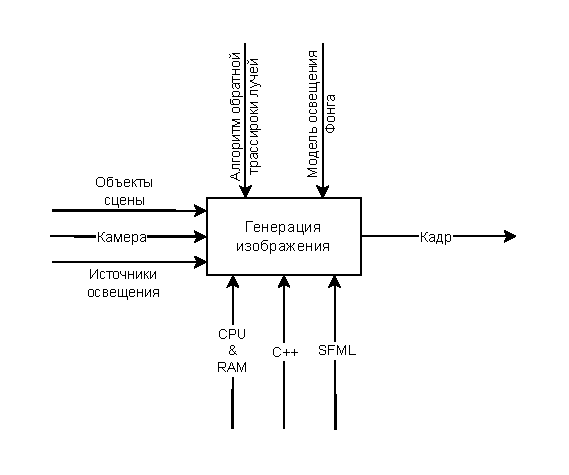
\includegraphics[width=1\textwidth]{IDEF0_specific.pdf}
    \caption{IDEF0 диаграмма верхнего уровня (A-0) выбранного для реализации алгоритма построения изображения}
    \label{fig:IDEF0_specific}
\end{figure}


\section{Алгоритм обратной трассировки лучей}
IDEF0 диаграмма уровня A-1 алгоритма трассировки лучей представлена на рисунке \ref{fig:IDEF0_trace_ray}.
\begin{figure}[H]
    \centering
    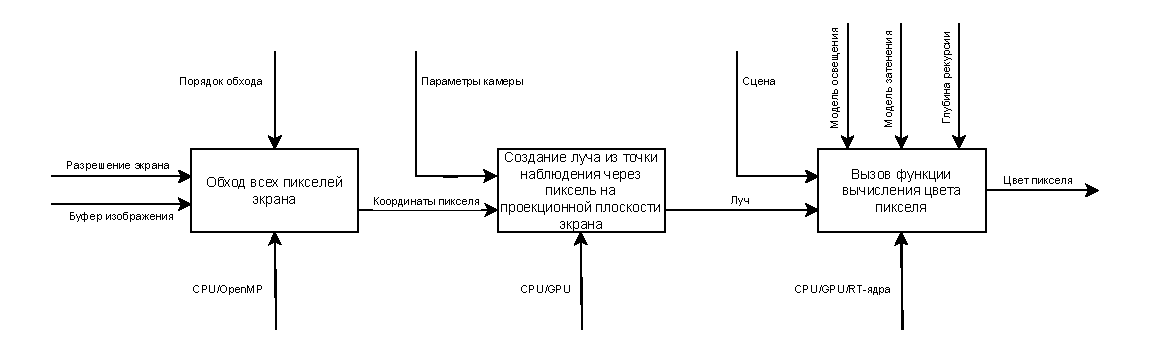
\includegraphics[width=0.8\textwidth]{IDEF0_RayTracing.pdf}
    \caption{IDEF0 диаграмма трассировки лучей}
    \label{fig:IDEF0_trace_ray}
\end{figure}

Схема алгоритма обратной трассироки лучей приведена на рисунке \ref{fig:trace_ray_diagram}.
\begin{figure}[H]
    \centering
    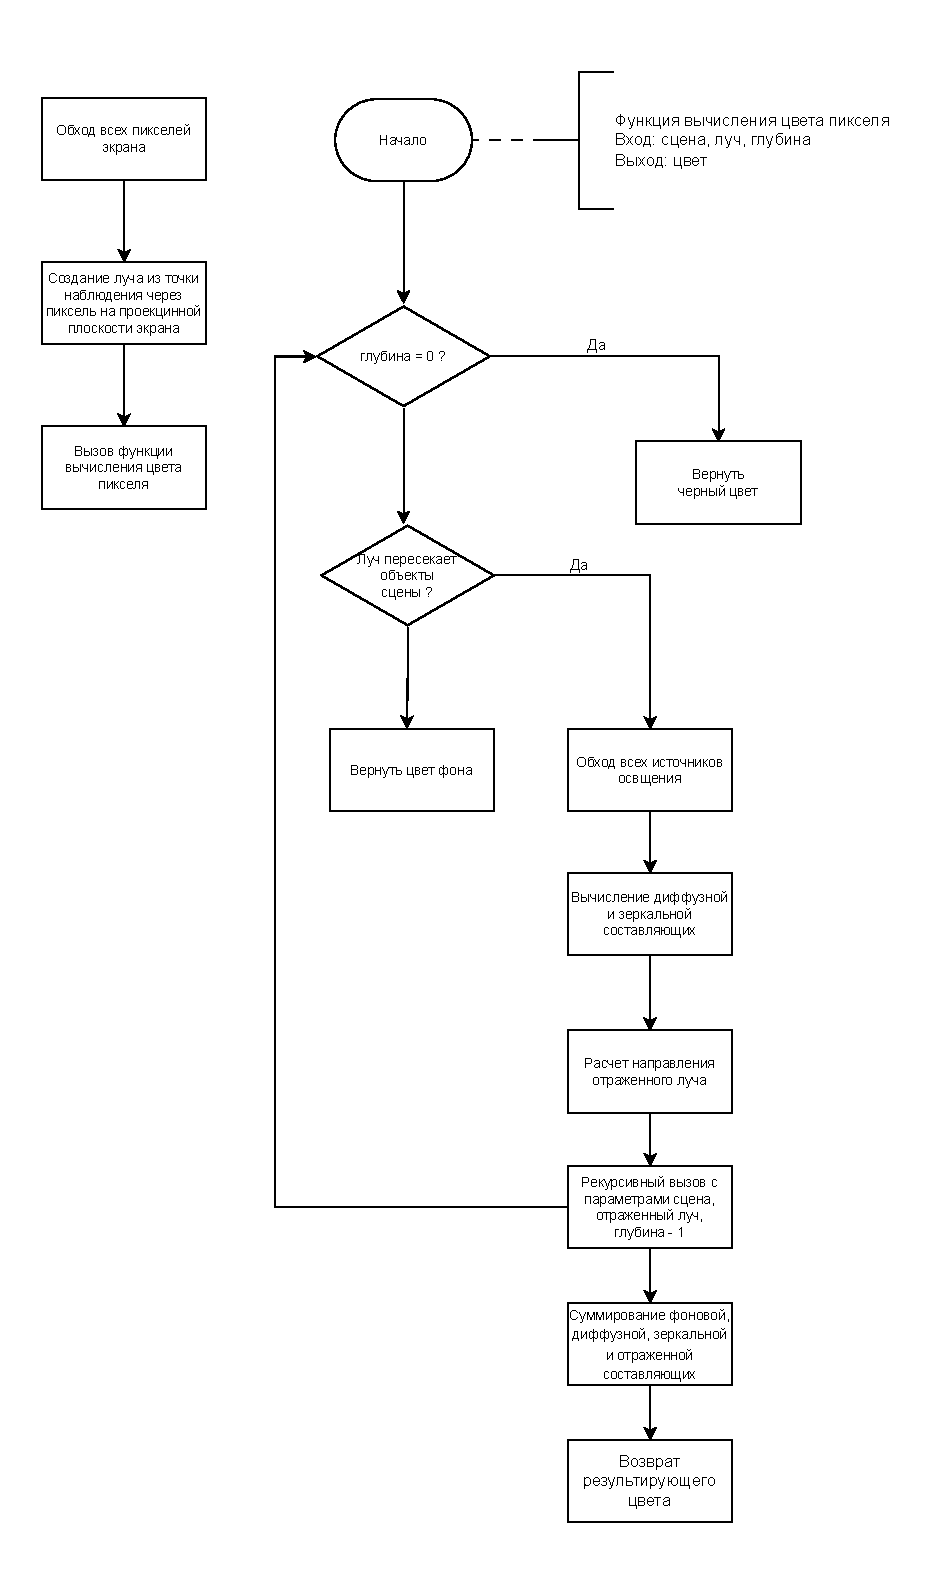
\includegraphics[width=0.6\textwidth]{trace_ray_diagram.pdf}
    \caption{Схема алгоритма обратной трассировки лучей}
    \label{fig:trace_ray_diagram}
\end{figure}
\chapter{Технологический раздел}

\section{Требования к ПО}
\section{Средства реализации}
C++, SFML, ImGui, CMake
\section{Типы и структуры данных}
Renderer, Scene, Camera, Object
Vec, Ray
\section{Алгоритмы}
\section{Графический пользовательский интерфейс}

% Многопоточность
\chapter{Исследовательский раздел}

\section{Анализ производительности ПО}

В качестве тестовой сцены для анализа времени генерации кадра был выбран чайник университета Юта (Utah Teapot)\cite{utah_teapot}, помещенный в Корнеллскую коробку (Cornell Box)\cite{cornell_box}. Для освещения был использован точечный источник, помещенный на середину потолка.

\noindent Тестовая сцена состоит из:
\begin{itemize}
    \item Корнеллской коробки;
    \item чайника Юта;
    \item точечного источника освещения.
\end{itemize}

\noindent Параметра генерации кадра:
\begin{itemize}
    \item разрешение кадра $1280\times720$ пикселей;
    \item максимальное число переотражений луча = 2.
\end{itemize}

\noindent Параметры системы, на которой будут проводиться замеры времени:
\begin{itemize}
    \item CPU -- 6C/12T @ 3.7GHz;
    \item RAM -- 32GB DDR5;
    \item OS -- Windows 11.
\end{itemize}

Для распараллеливания программы использовался стандарт OpenMP\cite{openmp}. Выбор обусловлен относительной простостой способа примения технологии. В языке C++ эта технология реализуется с помощью директивы \#pragma.

% \#pragma omp parallel for schedule(dynamic)

Для установки числа потоков используется функция \texttt{omp\_set\_num\_threads(int)} из заголовочного файла \texttt{<omp.h>}. Для получения количества логических ядер процессора используется функция \texttt{omp\_get\_max\_threads()}.

\begin{figure}[H]
    \centering
    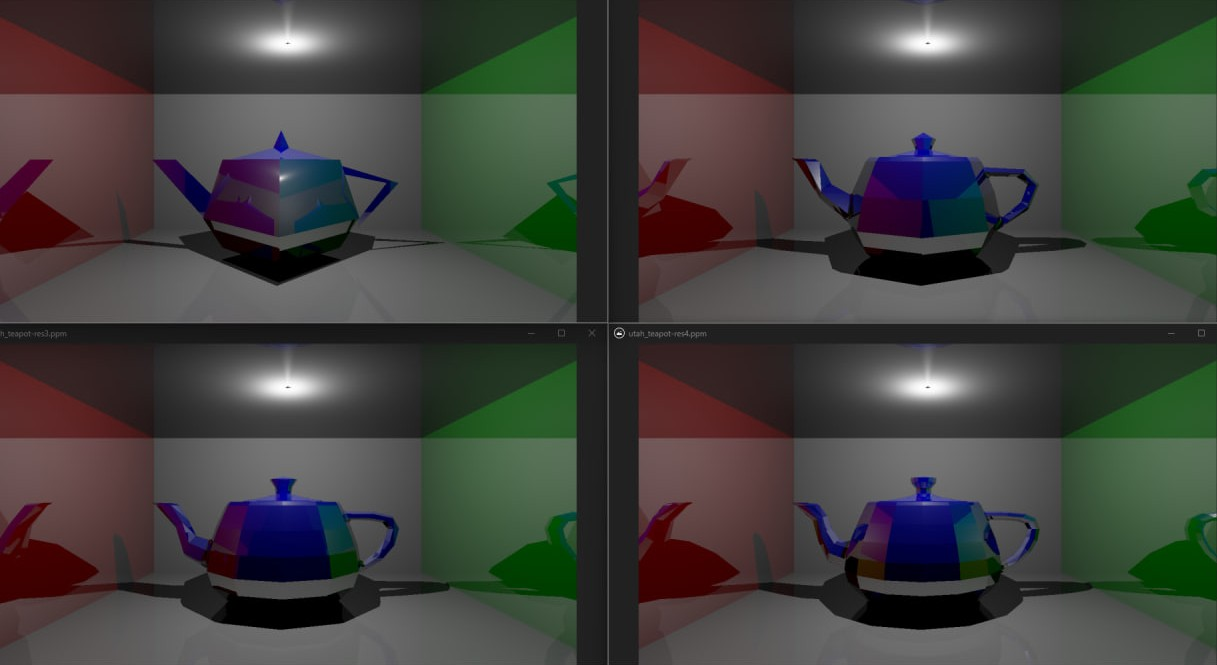
\includegraphics[width=1\textwidth]{utah-teapot.jpg}
    \caption{Чайники с разным числом полигонов}
    \label{fig:utah-teapot}
\end{figure}

Для исследования времени генерации кадра были выбраны следующие варианты числа потоков:
\begin{itemize}
    \item Однопоточный режим (1);
    \item Количество потоков, равное числу физических ядер процессора (6);
    \item Количество потоков, равное числу логических ядер процессора (12);
    \item Вдвое большее количество потоков по сравнению с числом логических ядер процессора (24).
\end{itemize}

Следующие графики представляют собой зависимость времени генерации изображения от количества граней в полигональной моделе чайника.

\begin{figure}[ht]
    \centering

    % 1 поток
    \begin{subfigure}[b]{0.45\textwidth}
        \centering
        \begin{tikzpicture}
            \begin{axis}[
                    title={1 поток},
                    xlabel={число граней},
                    ylabel={время (с)},
                    grid=major
                ]
                \addplot coordinates {
                        (108,15.351) (532,53.706) (1166,114.694) (2148,199.755)
                    };
            \end{axis}
        \end{tikzpicture}
    \end{subfigure}
    \hfill
    % 6 потоков
    \begin{subfigure}[b]{0.45\textwidth}
        \centering
        \begin{tikzpicture}
            \begin{axis}[
                    title={6 потоков},
                    xlabel={число граней},
                    ylabel={время (с)},
                    grid=major
                ]
                \addplot coordinates {
                        (108,4.505) (532,15.768) (1166,30.743) (2148,55.789)
                    };
            \end{axis}
        \end{tikzpicture}
    \end{subfigure}
    \hfill
    % 12 потоков
    \begin{subfigure}[b]{0.45\textwidth}
        \centering
        \begin{tikzpicture}
            \begin{axis}[
                    title={12 потоков},
                    xlabel={число граней},
                    ylabel={время (с)},
                    grid=major
                ]
                \addplot coordinates {
                        (108,2.818) (532,9.704) (1166,21.069) (2148,38.631)
                    };
            \end{axis}
        \end{tikzpicture}
    \end{subfigure}
    % 24 потока
    \begin{subfigure}[b]{0.45\textwidth}
        \centering
        \begin{tikzpicture}
            \begin{axis}[
                    title={24 потока},
                    xlabel={число граней},
                    ylabel={время (с)},
                    grid=major
                ]
                \addplot coordinates {
                        (108,2.566) (532,9.595) (1166,18.611) (2148,36.063)
                    };
            \end{axis}
        \end{tikzpicture}
    \end{subfigure}

    \caption{Время генерации кадра в зависимости от числа потоков и числа граней}
    \label{fig:all_plots}
\end{figure}

\begin{table}[ht]
    \centering
    \caption{Время генерации кадра в зависимости от числа потоков и числа граней}
    \begin{tabular}{|c|c|c|c|c|}
        \hline
        Число граней & 1 поток & 6 потока & 12 потоков & 24 потоков \\
        \hline
        108          & 15.4    & 4.5      & 2.5        & 2.6        \\
        532          & 53.7    & 15.8     & 8.8        & 9.6        \\
        1166         & 114.7   & 30.7     & 18.8       & 18.6       \\
        2148         & 199.8   & 55.8     & 38.6       & 36.1       \\
        \hline
    \end{tabular}
    \label{tab:frame_times_1dp}
\end{table}


На графике ниже представлена зависимость времени генерации кадра от числа потоков.

\begin{tikzpicture}
    \begin{axis}[
            title={Время генерация кадра в зависимости от числа потоков},
            xlabel={число потоков}, ylabel={время, (с)},
            grid=major
        ]
        \addplot[green, mark=o] coordinates {
                (1,15.351) (2,7.966) (4,4.505) (8,2.818) (12,2.488) (16,2.652) (20,2.515) (24,2.566)
            };

        \addplot[yellow, mark=*] coordinates {
                (1,53.706) (2,27.058) (4,15.768) (8,9.704) (12,8.803) (16,9.455) (20,8.843) (24,9.595)
            };

        \addplot[orange, mark=x] coordinates {
                (1,114.694) (2,57.741) (4,30.743) (8,21.069) (12,18.769) (16,19.316) (20,18.568) (24,18.611)
            };

        \addplot[red, mark=+] coordinates {
                (1,199.755) (2,105.847) (4,55.789) (8,38.631) (12,38.612) (16,33.443) (20,36.925) (24,36.063)
            };

        \legend{108 граней, 532 грани, 1166 граней, 2148 граней}
    \end{axis}
\end{tikzpicture}


\section*{Выводы}
Анализ представленных графиков позволяет сделать вывод, что прирост производительности с увеличением числа потоков носит ограниченный характер. Наиболее эффективным числом потоков является количество логических ядер процессора, при котором достигается максимальная параллельная загрузка. При дальнейшем увеличении числа потоков наблюдается снижение производительности, что связано с дополнительными затратами процессорного времени на переключение контекста между потоками.

% \section{Сравнение производительности на CPU/GPU}

% \section{Сравнение производительности без/с BVH}
% \section{Сравнение изображений, полученных с моделями освещения Ламберта/Фонга/Блинна-Фонга}
% \section{Сравнение изображений c разной гаммо-корреккций/тон-маппингом}


\chapter*{ЗАКЛЮЧЕНИЕ}
\addcontentsline{toc}{chapter}{ЗАКЛЮЧЕНИЕ}

В ходе выполнения курсовой работы все поставленные задачи были успешно решены, и цель работы достигнута. Разработанное ПО позволяет отображать сцены с геометрическими примитивами, поддерживает добавление и удаление объектов и источников света, позволяет изменять их положение и ориентацию, а также управлять положением и направлением камеры. Реализованный алгоритм трассировки лучей в сочетании с графическим интерфейсом обеспечивает корректную визуализацию сцены и удобство взаимодействия пользователя с программой.

\makebibliography

\begin{appendices}
	\chapter{Презентация к курсовой работе}
	Презентация содержит 12 слайдов.
	\chapter{Флешка с разработранным ПО}
	% TODO: структура файлов
\end{appendices}

\end{document}